%%%%%%%%%%%%%%%%%%%%%%%%%%%%%%%%%%%%%%%%%%%%%%%%%%%%%%%%%%%%%%%%%%%%
%% I, the copyright holder of this work, release this work into the
%% public domain. This applies worldwide. In some countries this may
%% not be legally possible; if so: I grant anyone the right to use
%% this work for any purpose, without any conditions, unless such
%% conditions are required by law.
%%%%%%%%%%%%%%%%%%%%%%%%%%%%%%%%%%%%%%%%%%%%%%%%%%%%%%%%%%%%%%%%%%%%

\documentclass{beamer}
\usetheme[faculty=fi]{fibeamer}
\usepackage[utf8]{inputenc}
\usepackage[
  main=english, %% By using `czech` or `slovak` as the main locale
                %% instead of `english`, you can typeset the
                %% presentation in either Czech or Slovak,
                %% respectively.
  				 %% The additional keys allow foreign texts to be
]{babel}   

%% These additional packages are used within the document:
\usepackage{ragged2e}  % `\justifying` text
\usepackage{booktabs}  % Tables
\usepackage{tabularx}
\usepackage{tikz}      % Diagrams
\usetikzlibrary{calc, shapes, backgrounds}
\usepackage{amsmath, amssymb}
\usepackage{url}       % `\url`s
\usepackage{listings}  % Code listings
\frenchspacing
\setbeamertemplate{frametitle}[default][center]
\begin{document}
  
 \begin{darkframes}
    \begin{frame}<beamer>
     \frametitle[alignment=center]{Monopoly}
      \begin{center}
		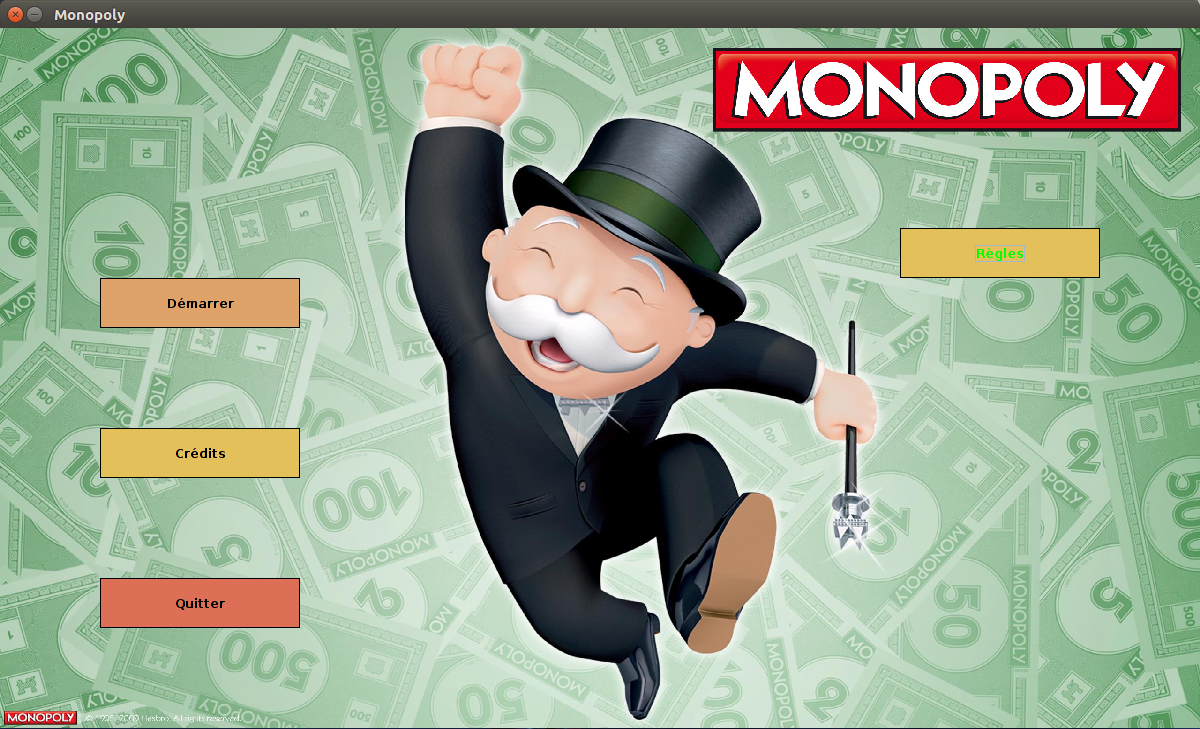
\includegraphics[scale=0.25]{./img/titre.png}
		
		\end{center}
		\vspace*{0.1cm}
		  \begin{center}
		Magniez Loïck
		\end{center}
    \end{frame}

    \begin{frame}<beamer>
      \frametitle{Table des Matières}
      \tableofcontents[]
    \end{frame}
    

 \section{Conception objet - UML}
 \begin{frame}
 	 \frametitle{UML MVC}
 	 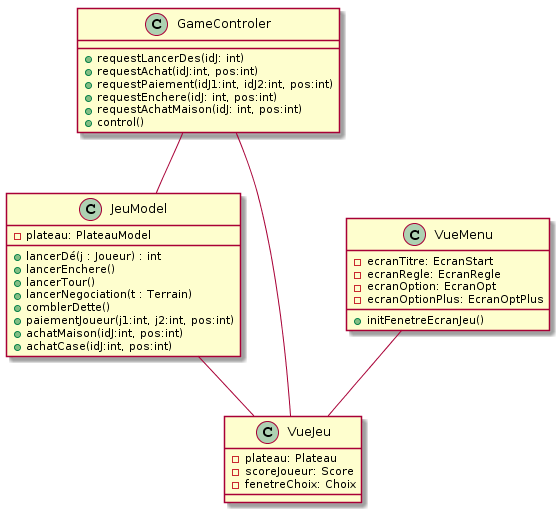
\includegraphics[scale=0.3]{./img/umlMVC.png}
 \end{frame}
 
 \begin{frame}
 	 \frametitle{UML du modèle}
 	 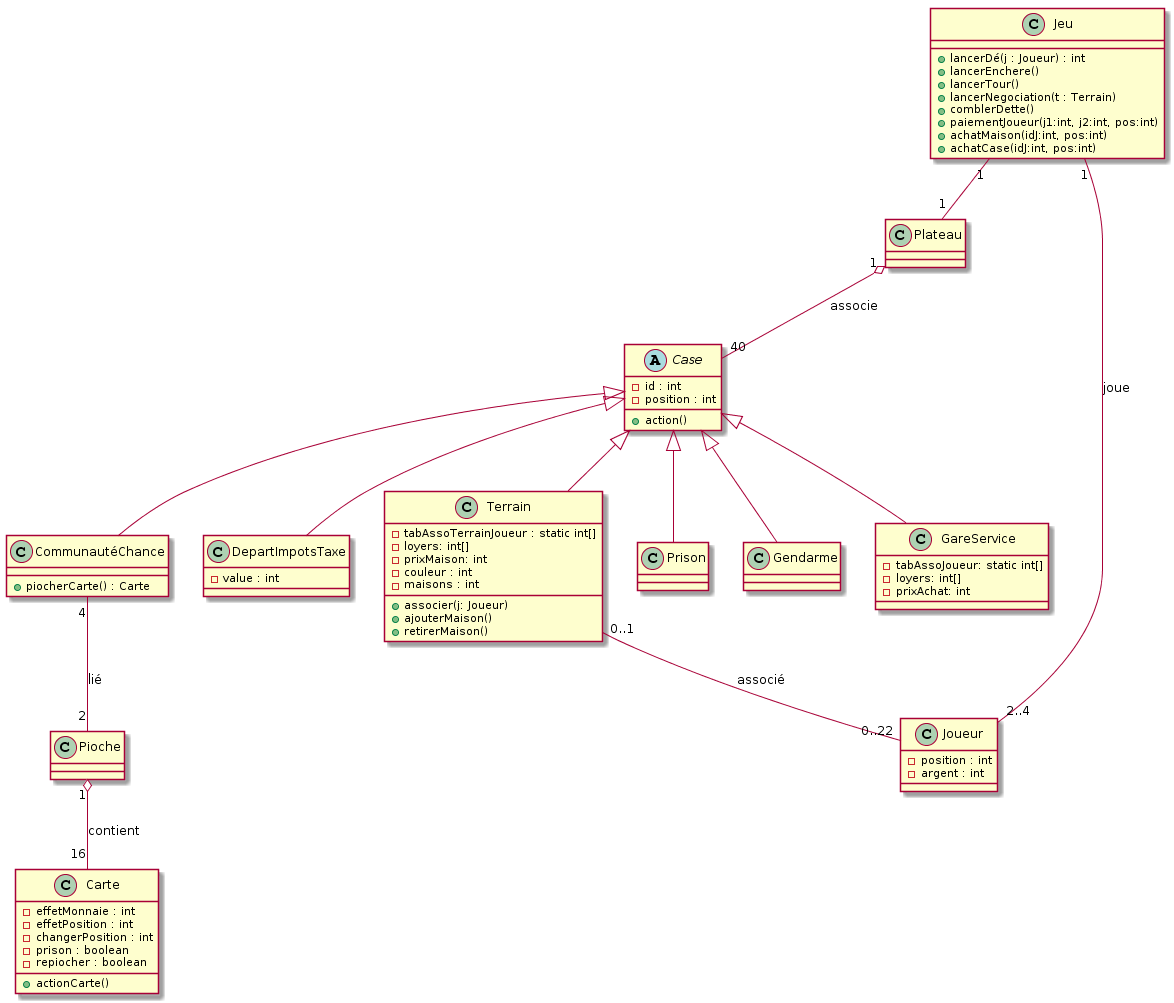
\includegraphics[scale=0.3]{./img/umlv2.png}
 \end{frame}
    
 \section{Ce qui a été réalisé}
	\subsection{Fonctionnalités générales} 	
 	\begin{frame}
 	 \frametitle{Fonctionnalités générales}
 	 
 	 
 	 	Génération du plateau simple, cases découpées et dessinées indépendamment.\\%
		Génération des événements simples de jeu :\\% 
		-Lancer un dé\\%
		-Acheter une propriété\\% 		
		-Payer un joueur\\% 
		-Ajouter une maison\\%
		-Vendre une propriété à un joueur\\%
 	 	
    \end{frame}
    
    \subsection{Paramétrage} 	
     \begin{frame}
 	 \frametitle{Paramétrage de la partie}
 	 \begin{center}
 	 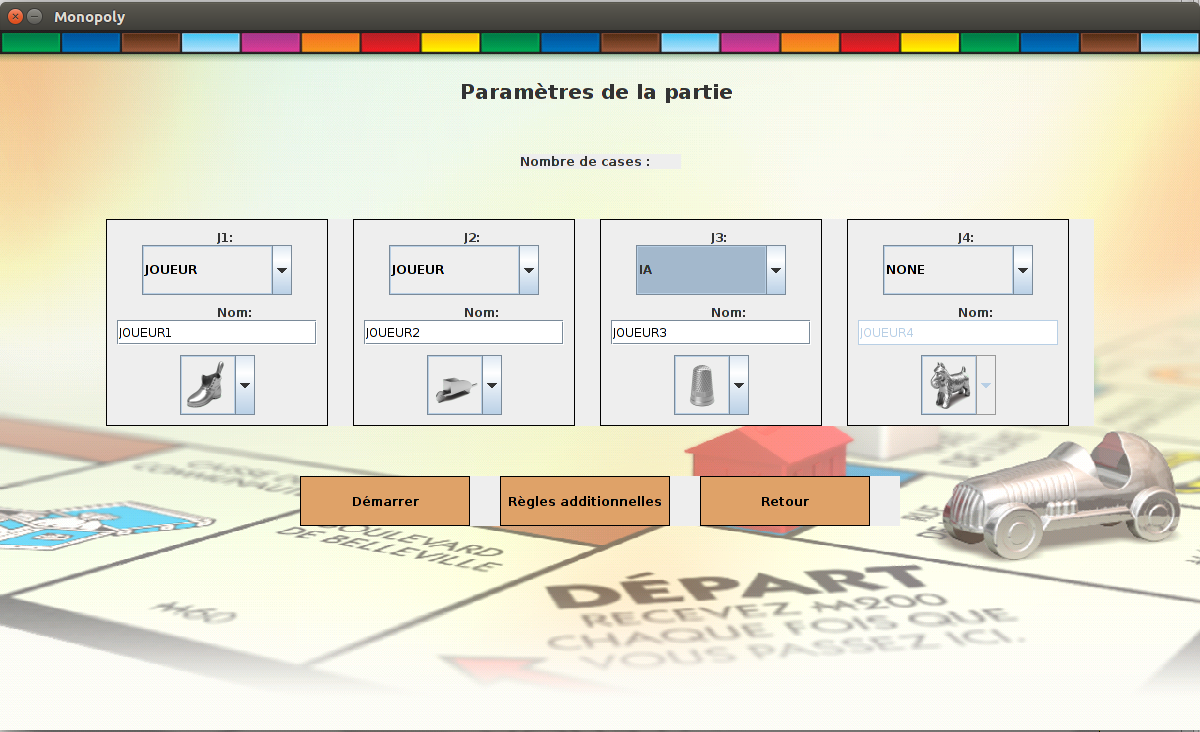
\includegraphics[scale=0.25]{./img/parametre1.png}
		
	\end{center}
    \end{frame}
    
    \begin{frame}
 	 \frametitle{Paramétrage avancé de la partie}
 	 \begin{center}
 	 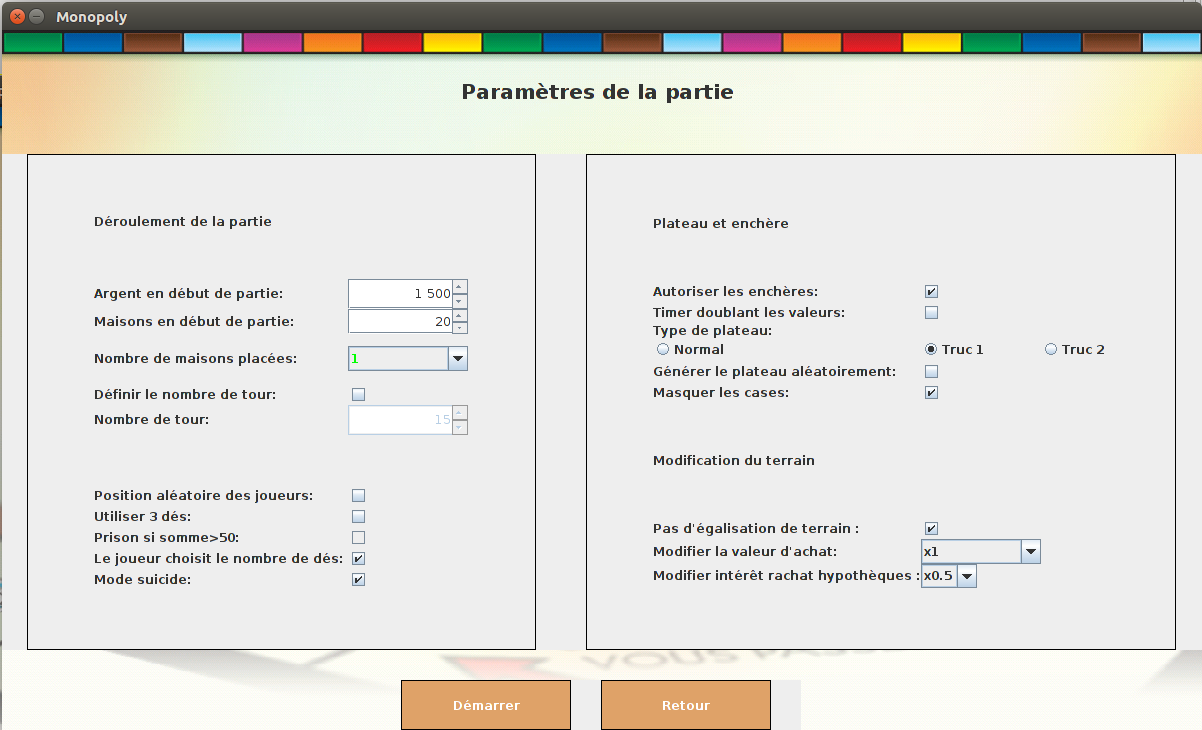
\includegraphics[scale=0.25]{./img/parametre2.png}
		
	\end{center}
    \end{frame}
  
	\subsection{Plateau} 	  
	\begin{frame}
 	 \frametitle{Plateau du jeu}
 	 \begin{center}
 	 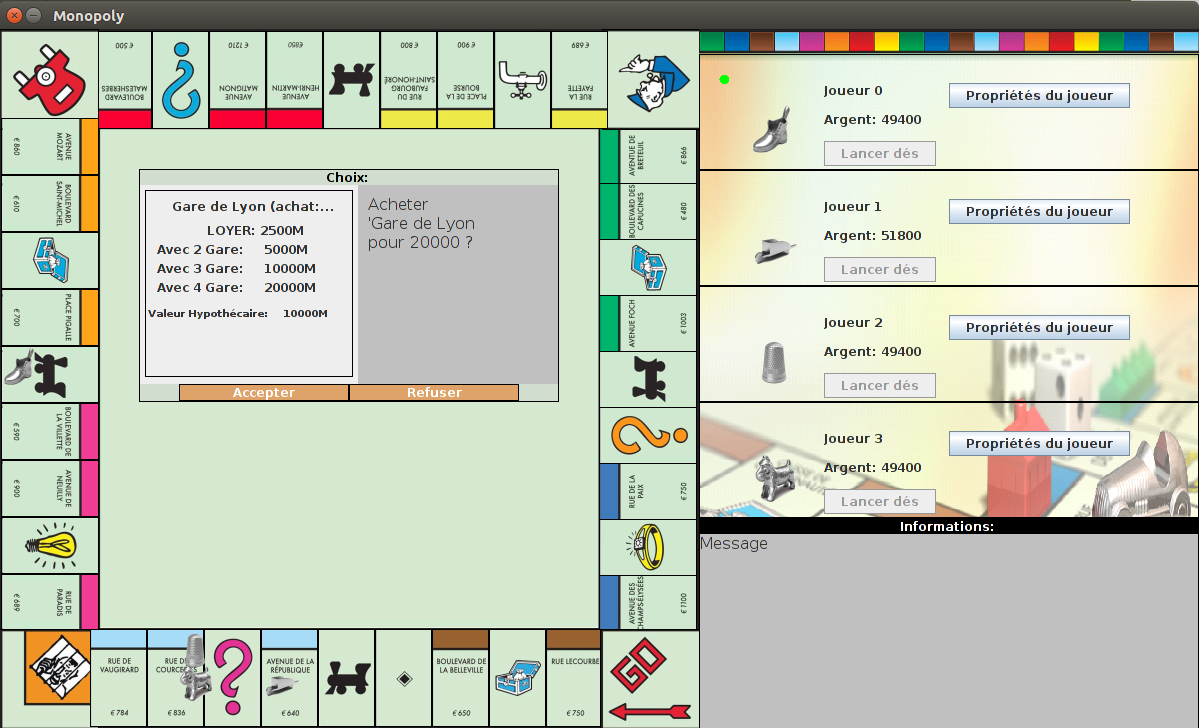
\includegraphics[scale=0.25]{./img/plateau.png}
		
	\end{center}
    \end{frame}	
	
	\subsection{Événements du jeu} 	  
  	\begin{frame}
 	 \frametitle{Événements}
 	 \begin{center}
 	 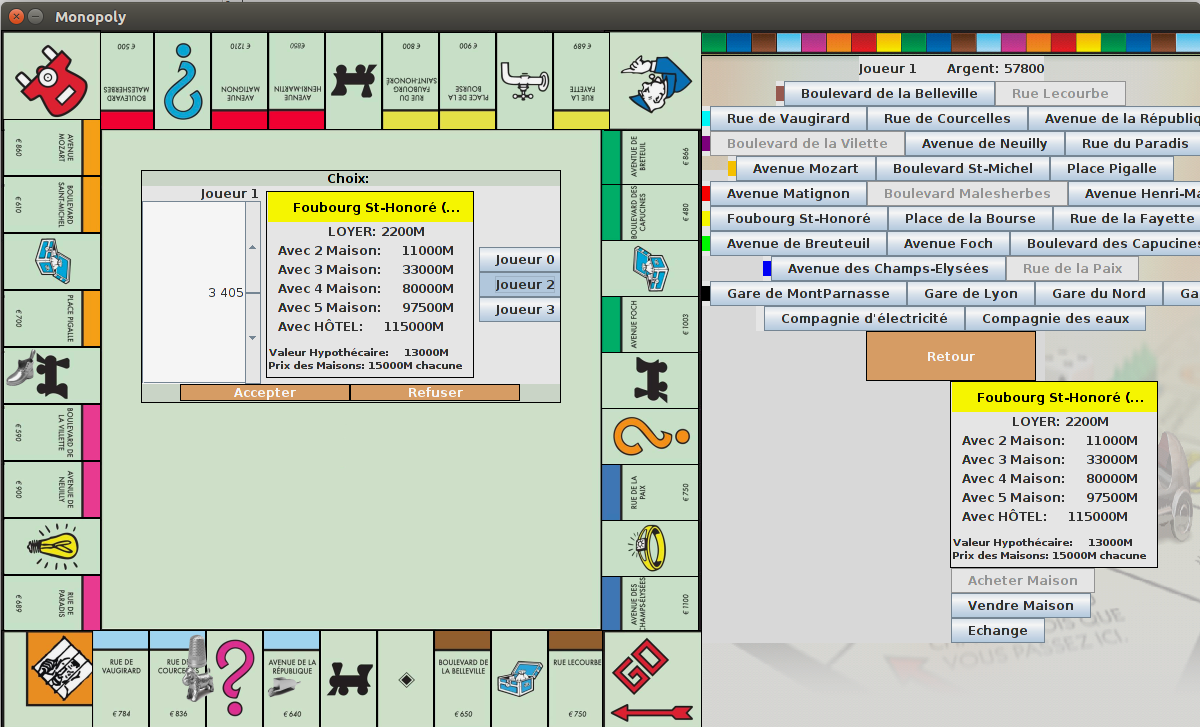
\includegraphics[scale=0.25]{./img/plateauInGame2.png}
		
	\end{center}
    \end{frame}	
    
    \begin{frame}
 	 \frametitle{Achat de case}
 	 \begin{center}
 	 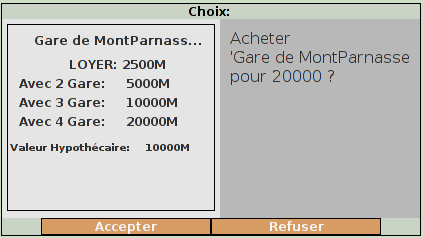
\includegraphics[scale=0.50]{./img/choixAchat.png}
		
	\end{center}
    \end{frame}
    
    \begin{frame}
 	 \frametitle{Paiement}
 	 \begin{center}
 	 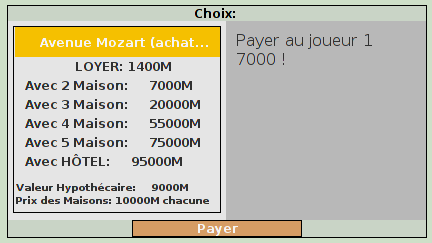
\includegraphics[scale=0.50]{./img/choixPaiement.png}
		
	\end{center}
    \end{frame}
    
    \begin{frame}
 	 \frametitle{Vente}
 	 \begin{center}
 	 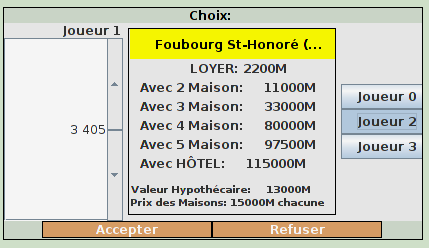
\includegraphics[scale=0.50]{./img/choixEchange.png}
		
	\end{center}
    \end{frame}
    
    \subsection{Interface joueur}
     \begin{frame}
 	 \frametitle{Écran score}
 	 \begin{center}
 	 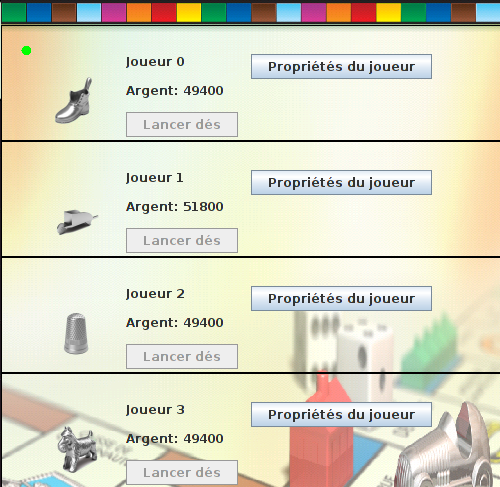
\includegraphics[scale=0.50]{./img/scoreJoueur.png}
		
	\end{center}
    \end{frame}
    
    \begin{frame}
 	 \frametitle{Propriétés du joueur}
 	 \begin{center}
 	 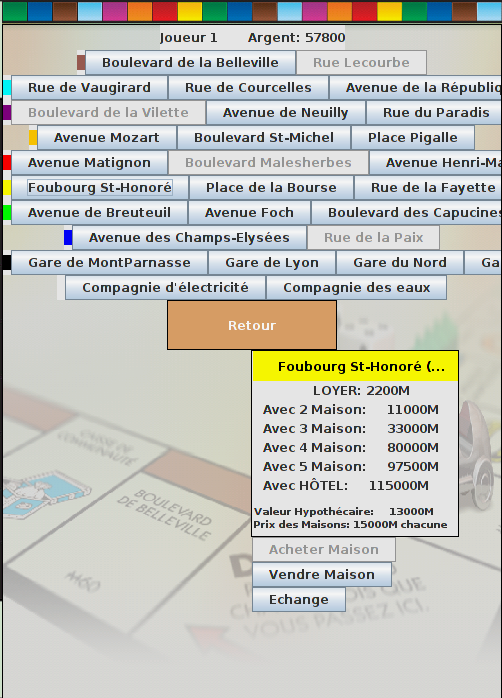
\includegraphics[scale=0.35]{./img/proprietes.png}
		
	\end{center}
    \end{frame}
	
	\subsection{Règles additionnelles}    
    \begin{frame}
 	 \frametitle{Écran score}
 	 \begin{center}
 	 Implémentation d'une partie des règles additionnelles
 	 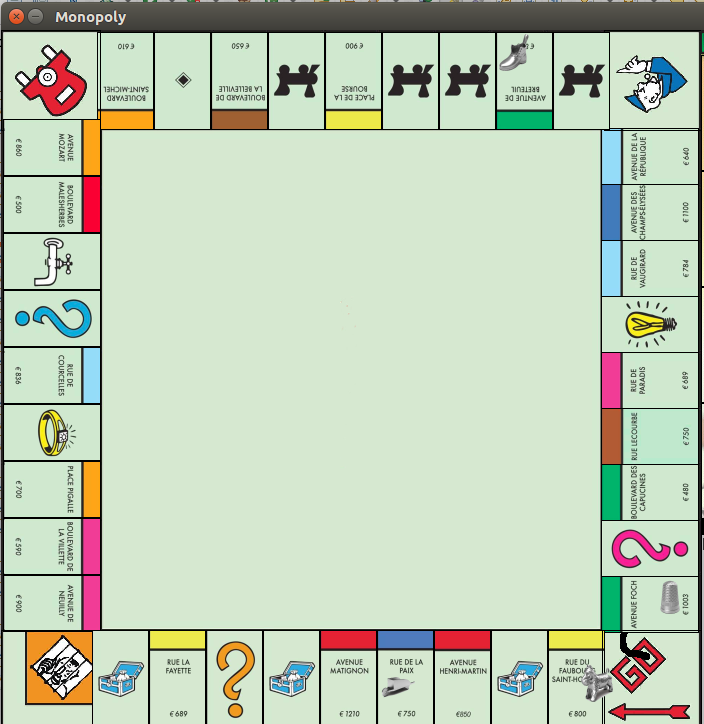
\includegraphics[scale=0.30]{./img/plateauAlea.png}
		
	\end{center}
    \end{frame}
    
\section{Ce qu'il reste à implémenter}    
	\begin{frame}
 	 \frametitle{Ce qu'il reste à implémenter}
 	 \begin{itemize}
\item Enchères
\item Prison
\item Carte chance
\item Déplacer en gare
\item Événement gagne
\item Sauvegarde XML
\end{itemize}

Toutes les règles supplémentaires :
\begin{itemize}
\item Cases cachées
\item ...
\end{itemize}
		
    \end{frame}    
    
    
         \section{Conclusion}
 \begin{frame}
   	 \begin{center}
  \Huge	 Conclusion
  		\end{center}
    \end{frame}
    
     \section{Les Questions}
 \begin{frame}
   	 \begin{center}
  	 \Huge	 Avez-vous des questions ?
  		\end{center}
    \end{frame}
    
  \end{darkframes}

\end{document}
